\section{Optimization}
\label{sec:eval_optimization}
The first aspect of our compiler we want to evaluate are the optimizations that are applied to the quantum circuit by the compiler. For this, we apply our optimizations to variants of the same algorithm, the quantum ripple-carry adder. Firstly, we analyze the optimizations to the adder when given classical inputs. Next, we evaluate the optimization of the adder for inputs in superposition with different register sizes. Lastly, we compare our optimizations to optimizations that are applied by the default quiskit transpilation process of quantum circuits.

In our first example, we use the inputs $a = \ket{1}$ and $b = \ket{15}$ with both the input and output carry qubit having a value of $\ket{0}$. Furthermore, both input registers have a size of 4 qubits and, in turn, have $2^4 = 16$ possible classical values. After the adder is applied, the $a$ register and carry input, per definition, remain at their initial values of $\ket{1}$ and $\ket{0}$ respectively. In contrast, the $b$ register now has a value of $\ket{0}$ and the carry output a value of $\ket{1}$, indicating that the result of the addition is $16$. 
The quantum circuit corresponding to the example before optimization rules are applied is depicted in Fig.~\ref*{fig:eval_adder_circuit}.\change{change to graphic without parallization}
\begin{figure}[htp]
    \centering     
    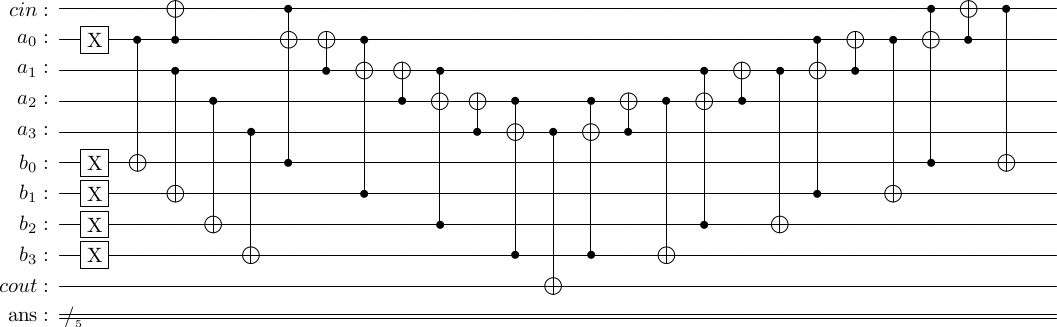
\includegraphics[width=\textwidth]{../figures/images/adderCircuit.png}
    \caption{An unoptimized circuit of a quantum ripple-carry adder.}
    \label{fig:eval_adder_circuit}
\end{figure}

Since the circuit only consists of $X$, controlled-not, and Toffoli gates, neither the Hadamard reductions nor control reversion optimization rules can be applied to the circuit. However, both the peeping control and null gate optimizations can be applied. Whenever a qubit wire contains a know value of $\ket{0}$,  the controlled gates can be remove. For the opposite case, the control can be removed and the resulting $X$ gate can be removed when in combination with another null gate. In turn, the circuit can be optimized such that the resulting one only contains gates that initialize the result; only two $X$ gates remain. While the first flips the first qubit of the $a$ register, initializing it to $\ket{1}$, the second flips the carry output qubit, indicating a result of $\ket{16}$. The OpenQASM code for the optimized circuit is depicted in App.~\ref{appendix:classicalInputs_optimized}.

In the second example, we input a value in superposition. Now, register $a$ contains a value of $\frac{1}{\sqrt{2}} (\ket{1} + \ket{3})$ and register $b$ contains a value of $\ket{4}$. Again, both carry qubits are initialized to $\ket{0}$. After the adder gate is applied, the carry qubits and register $a$ remain as initialized. However, the $b$ register now has a value of $\frac{1}{\sqrt{2}} (\ket{5} + \ket{8})$.
Since the input is now no longer a classical value, the peeping control optimization can only be applied in a few cases. In turn, only four gate are removed and four Toffoli gate are optimized to controlled-not gates.
The optimized quantum program is depicted in App.~\ref{appendix:superposInputs_optimized}. While the optimizations are not as effective for inputs in superpositions, they can optimize significant parts of the program. For example, when we repeat the same example but increase the size of both register to $64$ qubits, the optimized circuit contains the same amount of gates. In this case, all gate applications to qubit wires outside the influence of the data in superposition can be removed.\improvement{bad formulation}

We also compared the optimizations applied by our compiler to the default optimizations that are applied by the Qiskit transpilation process. Qiskit\footnote{\url{https://github.com/Qiskit/qiskit/}}~\cite{JTK*24} is a software development kit for building, simulating, and transpiling quantum circuits. Additionally, the kit can interpret OpenQASM programs and build quantum circuits from them. When transpiling quantum circuits with Qiskit, \ie transforming to a specific domain, \eg another basis gate set, the kit can perform optimizations to the circuit based on a optimization level. For the comparison, we wrote a OpenQASM program which applied the quantum ripple-carry adder. The code for the program is depicted in Fig.~\ref*{fig:eval_adder_qasm}. The program can then be loaded with Qiskit and build into a quantum circuit. To apply the default optimizations of Qiskit, we transpile the circuit with the highest optimization level to the basis gate set our compiler translates to, \ie $\{X, Y, Z, CX, CCX, H\}$. While our compiler translates to arbitrary controlled gates, they are not used in this example. Furthermore even the $Y$, $Z$, and Hadamard gate are redundant as they are not used.

\begin{figure}[htp]
    \centering     
    \lstinputlisting[style=QASM]{../figures/code/evaluation/adder.qasm}
    \caption{An OpenQASM 3 implementation of a quantum ripple-carry adder circuit.}
    \label{fig:eval_adder_qasm}
\end{figure}

However, while the Qiskit transpilation can apply many optimizations such as null gate optimizations, the default rule do not contain a rule similar to our peeping control optimization rule. In turn, no controlled gates can be optimized in the circuit. Furthermore, since the null gate optimizations can only be applied after peeping control rules were applied in our example, the transpilation process does not apply any optimizations to the circuit. Since Qiskit target lower level transpilation to specific hardware or quantum devises and not high level optimizations, its focus is on different optimizations. In contrast, our compiler has no transpilation capabilities and cannot target any specific hardware. In turn, the optimizations and overall capabilities of Qiskit and our compiler are complementary and can be used in tandem.
